\section{Конструкторская часть}

В данном разделе описываются используемые структуры данных, проводится подробное описание алгоритма оптимизации динамической трансляции доступа к памяти и сопутствующих ему алгоритмов. Проводится проектирование программной реализации алгоритма оптимизации динамической трансляции доступа к памяти.

Алгоритм рассчитан на организацию кода в блоки из которых одна точка выхода в конце блока и одна точка входа --- в начале блока.

\subsection{Архитектура программного обеспечения}

На высоком уровне трансляция в FEX проводится в 4 этапа. На рисунке \ref{fig:trans} представлена диаграмма трансляции.

\begin{figure}[hbtp]
	\centering
	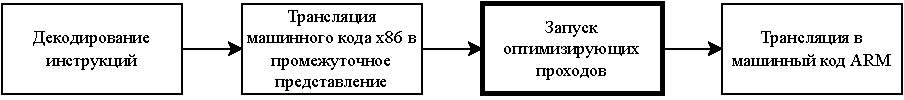
\includegraphics[width=\textwidth]{img/scale.pdf}
	\caption{Процесс трансляции программы в FEX}
	\label{fig:trans}
\end{figure}

Разработанный алгоритм --- это оптимизирующий проход, он вызывается во время запуска оптимизирующих проходов и работает с промежуточным представлением.

\subsection{Используемые структуры данных}

$BlockInfo$ --- структура хранящая информацию об отдельном блоке транслированного кода. Включает в себя:

\begin{itemize}[leftmargin=1.6\parindent]
	\item[---] $State$ --- рассчитанное состояние блока, свидетельствует о состоянии регистра RBP, либо регистр не менялся, либо в нем адрес связанный со стеком, либо в нем адрес не связанный со стеком. Может принимать значения: ON\_STACK, NOT\_STACK, NOT\_CHANGED.
	\item[---] $StackNodes$ --- множество операций загружающих стековое значение;
	\item[---] $UnStackNodes$ --- множество операций загружающих не стековое значение;
	\item[---] $Predecessors$ --- множество блоков трансляции предшествующих этому;
	\item[---] $Visited$ --- флаг, показывает обработан ли блок.
\end{itemize}

Из $BlockInfo$ создается словарь содержащий информацию по всем блокам трансляции которые были поданы в функцию.

$OrderedNode$ --- класс описывающий индивидуальную инструкцию, является членом двухсвязного списка:

\begin{itemize}[leftmargin=1.6\parindent]
	\item[---] $Header$ --- заголовок содержащий информацию об инструкции, ее операндах и прочее. Так же включает в себя указатели на предыдущую и последующую $OrderedNode$.
	\item[---] $NumUses$ --- счетчик использования инструкции.;
\end{itemize}

Блок трансляции --- это множество последовательных $OrderedNode$ оканчивающихся потерей управления.

%можно UML

%лучше это все в картинки перевести

\subsection{Алгоритм оптимизации динамической трансляции доступа к памяти}

\textbf{Входные данные:} Множество блоков транслированного кода $IRBlocks$.

\textbf{Выходные данные:} Множество блоков транслированного кода $IRBlocks$ с оптимизированным доступом к памяти.

\begin{algorithm}[H]
\small
	\caption{Алгоритм оптимизации динамической трансляции доступа к памяти}
	\label{alg:memopt}
	\begin{algorithmic}[1]
		\State $in$ $\gets$ множество блоков транслированного кода $IRBlocks$
		\State $out$ $\gets$ множество блоков транслированного кода с оптимизированным доступом к памяти $IRBlocks$
		\State $ControlFlow$ $\gets$ построить граф потока выполнения блоков
		\For{$i$ in $in$}
		\State $StackStatus$ $\gets$ NOT\_CHANGED \Comment{может принимать значения NOT\_CHANGED, ON\_STACK и NOT\_STACK}
		\For{$j$ in предшевственники $i$}
		\State $PredecessorState$ $\gets$ рассчитать состояние блока с учетом предшественников
		\If {$PredecessorState$ = ON\_STACK}
		\State $StackStatus$ $\gets$ $PredecessorState$
		\EndIf
		\If {$PredecessorState$ $\neq$ NOT\_STACK}
		\State $StackStatus$ $\gets$ $PredecessorState$
		\State $\mathbf{break}$
		\EndIf
		\EndFor
		\For{$CodeNode$ in строки кода $i$}
		\If {$CodeNode$ = инструкция загрузки адреса стека в RBP}
		\State $StackStatus$ $\gets$ ON\_STACK
		\EndIf
		\If {$CodeNode$ = инструкция загрузки любого значения, кроме стека в RBP}
		\State $StackStatus$ $\gets$ NOT\_STACK
		\EndIf
		\If {$StackStatus$ == ON\_STACK \textbf{and} $CodeNode$ = инструкция записи или чтения по адресу регистра RBP}
		\State $out$ $\gets$ заменить барьерную инструкцию на обычную
		\EndIf
		\EndFor
		\EndFor
	\end{algorithmic}
\end{algorithm}

\subsection{Алгоритм построения графа выполнения блоков}

\textbf{Входные данные:} Множество блоков транслированного кода $IRBlocks$.

\textbf{Выходные данные:} Ориентированный граф потока выполнения блоков $Predecessors$.

\begin{algorithm}[H]
\small
	\caption{Алгоритм построения графа выполнения блоков}
	\label{alg:graph}
	\begin{algorithmic}[1]
		\State $in$ $\gets$ множество блоков транслированного кода
		\State $Predecessors$ $\gets$ ориентированный граф потока выполнения блоков
		\State $State$ $\gets$ множество состояний блоков
		\State $StackNodes$ $\gets$ множество строк изменяющих содержимое регистра RBP на значение связанное с RSP
		\State $UnStackNodes$ $\gets$ множество строк изменяющих содержимое регистра RBP на значение не связанное с RSP
		\For{$i$ in $in$}
		\For{$j$ in строки $i$}
		\If {$j$ --- условный переход}
		\State $Predecessors$ $\gets$ i --- предшественник блоков куда передается управление
		\EndIf
		\If {$j$ --- безусловный переход}
		\State $Predecessors$ $\gets$ i --- предшественник правдивого блока куда передается управление
		\State $Predecessors$ $\gets$ i --- предшественник ложного блока куда передается управление
		\EndIf
		\If {$j$ --- запись регистра RBP}
		\If {записывается связанное с RSP значение}
		\State $State$ $\gets$ в блоке стековое значение
		\State $StackNodes$ $\gets$ строка записи стекового значения
		\Else
		\State $State$ $\gets$ в блоке не стековое значение
		\State $UnStackNodes$ $\gets$ строка записи не стекового значения
		\EndIf
		\EndIf
		\EndFor
		\EndFor
	\end{algorithmic}
\end{algorithm}

\subsection{Алгоритм расчета распространенного состояния стека}

Этот алгоритм используется для определения состояния регистра в последующих блоках. Если в блоке 1 была произведена загрузка стекового значения в регистр RBP, а в блоке 2, для которого предок только блок 1, этот регистр не меняется, то для всех потомков блока 2 следует считать что регистр содержит стековое значение.

\textbf{Входные данные:} Блоков транслированного кода $IRBlocks$, ориентированный граф потока выполнения блоков $ControlFlow$.

\textbf{Выходные данные:} Состояние блока с учетом предшественников.

\begin{algorithm}[H]
\small
	\caption{Алгоритм расчета распространенного состояния стека}
	\label{alg:bilin}
	\begin{algorithmic}[1]
		\State $TargetBlock$ $\gets$ блок для которого рассчитывается состояние стека
		\State $ControlFlow$ $\gets$ граф потока выполнения блоков
		\State $ResultingState$ $\gets$ состояния стека для блока с учетом предыдущих
		\State $out$ $\gets$ ON\_STACK
		\For{$i$ in предшественники $TargetBlock$}
		\State $PredecessorState$ $\gets$ рассчитать распространенное состояние стека для $i$
		\If {$PredecessorState$ = NOT\_CHANGED}
		\State $ResultingState$ $\gets$ NOT\_CHANGED
		\EndIf
		\If {$PredecessorState$ = NOT\_STACK}
		\State $ResultingState$ $\gets$ NOT\_STACK
		\State \textbf{break}
		\EndIf
		\EndFor
	\end{algorithmic}
\end{algorithm}

\subsection{Вывод}

Были описаны используемые структуры данных, дано описание используемых алгоритмов. Был спроектирован алгоритм оптимизации динамической трансляции доступа к памяти и сопутствующие ему алгоритмы.

\pagebreak